\documentclass{report}
\usepackage{graphicx}
\usepackage{framed}
\usepackage{verbatim}
\usepackage[section]{placeins}
\usepackage{titlesec}
\newcommand{\sectionbreak}{\clearpage}
\usepackage{hyperref}
\usepackage{fixlatvian}
\usepackage{circuitikz}
\usepackage{tikz}
\usepackage{pgfplots}
\pgfplotsset{compat=1.15}
\graphicspath{ {images/} }
\title{Labaratorijas darba 1. atskaite}
\author{Artjoms Ivanovs}
\date{March 2018}
\begin{document}
\maketitle
\chapter{Teorētiska daļa}
Sprieguma avota V1 sprieguma vērtību U (Voltos) izvēlejos daļskaitli, kas ir apliecības pēdējie trīs cipari dalīti ar
10.\cite{a_1}
Piemēram. ‘171REB146’ nozīmē V1 = 14.6 (Volti), R1 ir apliecības pēdējo 3 ciparu otrais
numurs+1, R2 ir apliecības numura pēdējais cipars +1. Piemēram, ja apliecības numurs
ir ‘171REB146’ tad ‘R1=5’, ‘R2=7’\cite{a_2}

\begin{center}
\begin{circuitikz}[american voltages]
\draw
  (0,0.7) to [short] (5,0.7)
  to [V] (5,2) 
  to [R] (5,4) 
  to [short] (4,4) 
  (0,0.7) to [open] (0,0.7) 
  to [short] (0,4) 
  to [R] (4,4);
  \end{circuitikz}
  \end{center}
\begin{figure}
\begin{center}
\begin{tikzpicture}
\begin{axis}[
    xlabel=$R2$,
    ylabel=$U_{R2}$
    ]
\addplot[color=red,mark=*] coordinates {
		(5.22,7.35)
		(5.44,7.40)
		(5.67,7.48)
		(5.89,7.55)
		(6.11,7.65)
		(6.33,7.75)
		(6.55,7.82)
		(6.77,7.9)
		(6.99,7.95)
	};
\end{axis}
\end{tikzpicture}
\caption{$U_{R2}$=\textit{f}(\textit{R2}) grafiks, pēc sweep simulācijas datiem.}\label{graph:1}
\end{center}
\end{figure}


\section{Ķēdes aprēķins}
\begin {table}[h]
\begin{tabular}{|c|c|}
\hline
$R_1$ & 5\\
\hline
$R_2$ & 7  \\
\hline
$V_1$ & 14.6  \\
\hline
$U_{R1}$ & 14.6  \\
\hline
$U_{R2}$ & 8.52  \\
\hline

\end{tabular}
\caption {Sprieguma un pretestības tabula}
\end {table}
\begin{figure}[h]
    \centering
    \rotatebox{-90}{\includegraphics[scale=1, trim={7cm 8cm 11cm 14cm},clip]{01.ps}}
    \caption{Shēma}
    \label{fig:my_label1}
\end{figure}

\chapter{Praktiska daļa}
\section{Darbs ar GEDA programmām}
    \subsection{Darbs ar gschem}

        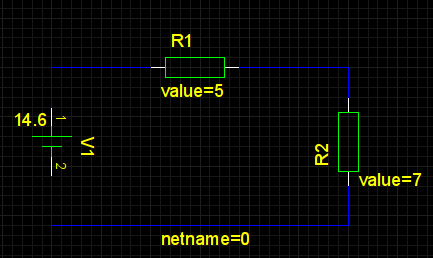
\includegraphics[width=12cm, height=6cm]{2.png}

\captionof{figure}{Elektriska shēma gschem vidē}
    \subsection{Darbs ar gnetlist}

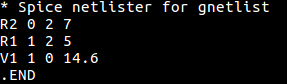
\includegraphics[width=5cm, height=2cm]{3.png}
\captionof{figure}{Rezultātu parbaude ar gnetlist}

\subsection{Darbs ar ngspice}
    \begin{figure}[h]
        \centering
        \rotatebox{0}{{\frame{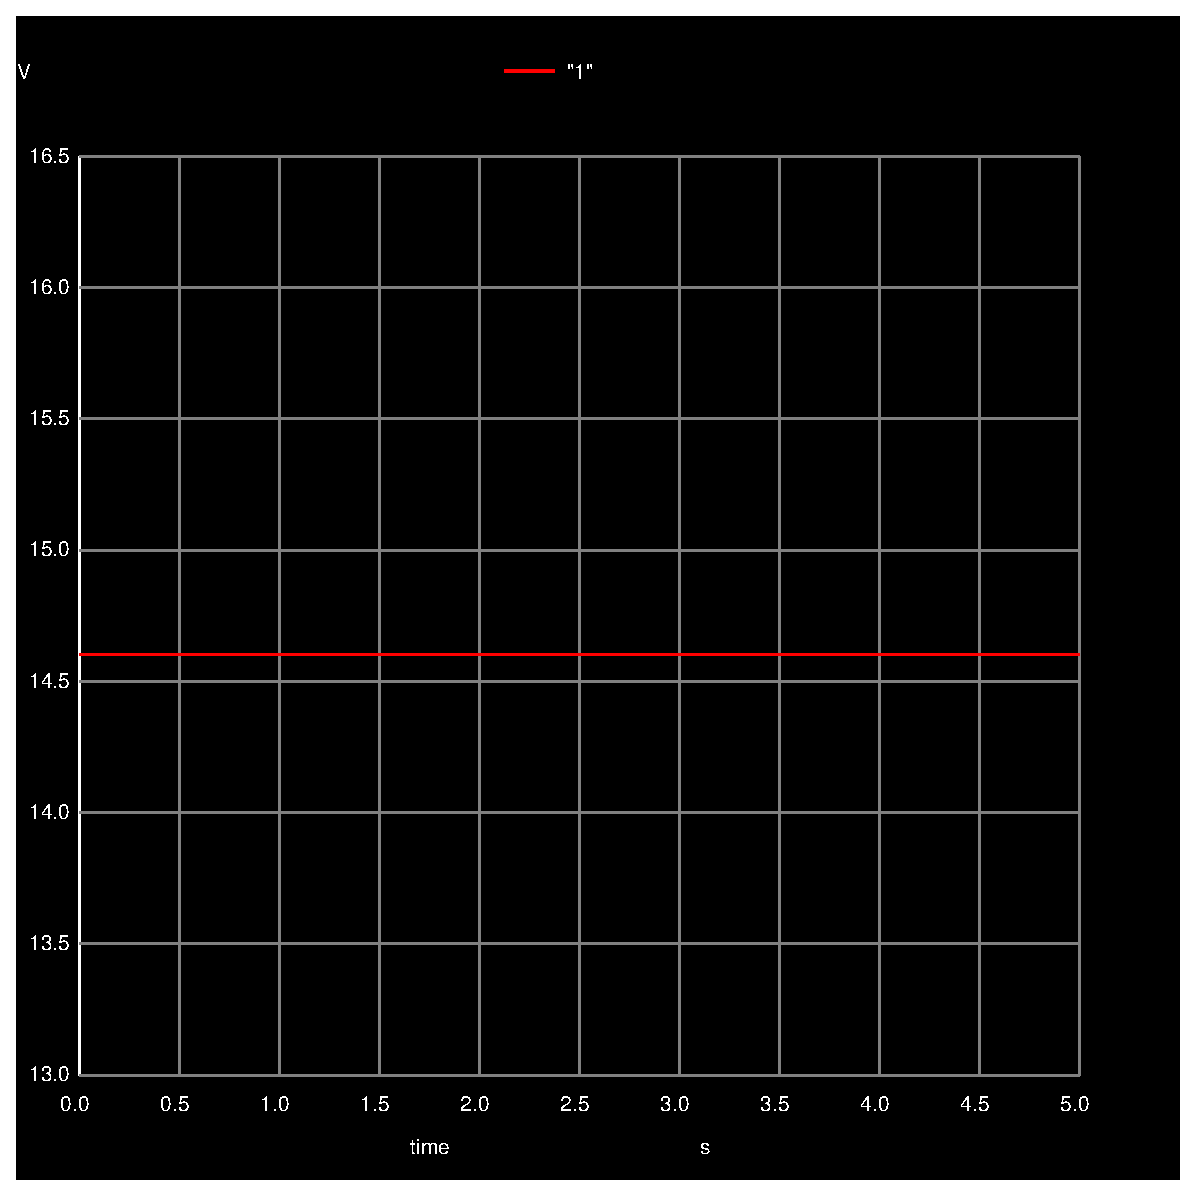
\includegraphics[scale=0.32]{011.ps}}}}
        \label{fig:my_label2}
    \end{figure}
    \begin{figure}[h]
         \centering
        \rotatebox{0}{{\frame{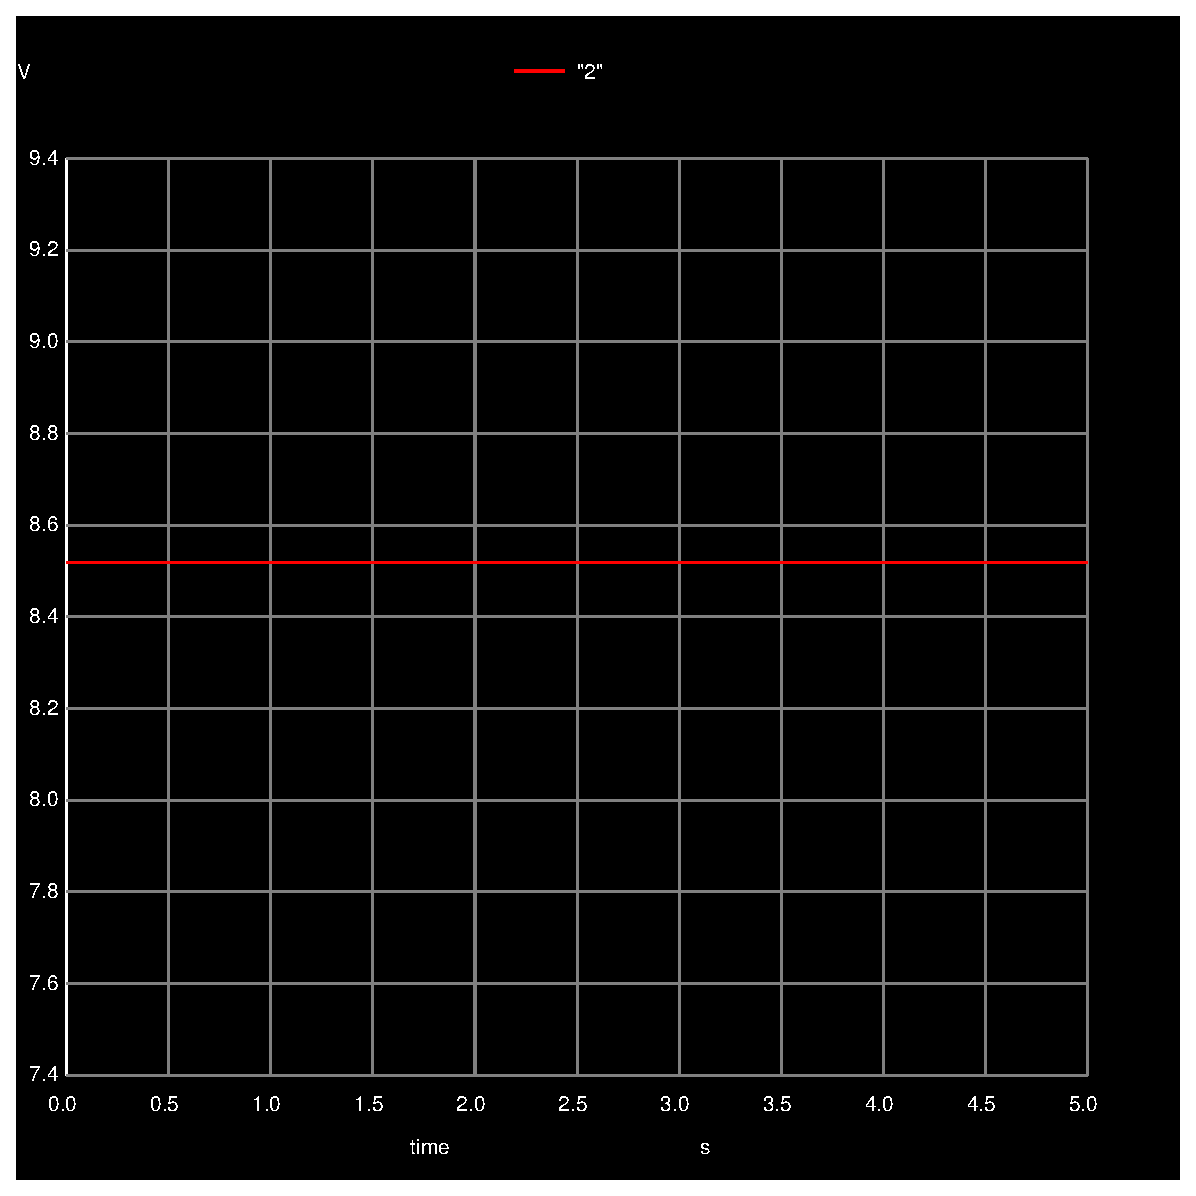
\includegraphics[scale=0.32]{012.ps}}}}
        \caption{NGspice iegūtaie sprieguma grafiki}
        \label{fig:my_label3}
    \end{figure}
\section{Darbs ar QUCS programmām}
    \begin{figure}[h]
        \centering
        \rotatebox{-90}{{\frame{\includegraphics[scale=1.2, trim={1cm 1cm 16cm 21cm},clip]{similation.ps}}}}
        \caption{QUCS Shēmas modelis}
        \label{fig:my_label4}
    \end{figure}
    \subsection{Tabula un grafiks}
    \begin{figure}[h]
        \centering
        \rotatebox{-90}{\frame{\includegraphics[scale=1.5, trim={1cm 1cm 17cm 18cm},clip]{grafiki.ps}}}
        \caption{Iegūtie rezultāti QUCS}
        \label{fig:my_label5}
    \end{figure}
\begin{thebibliography}{9}
\bibitem{a_1}
Berga, I,. Ceske, E., Čekstere, I. u.c. 
\textit{Siguldas novadmācība}. (Latvia) 
[\textit{Siguldas novadmācība}]
Berga, I,. Ceske, E., Čekstere, I. u.c. Rīga: Preses nams, 2002. 186 lpp. ISBN 9984-19-250-4.

\bibitem{a_2} 
Joseph Heller
\textit{Catch-22}. 
Published September 4th 2004 by Simon and Schuster (first published 1961)
\end{thebibliography}

\end{document}
